%!TEX root = ../dokumentation.tex

\chapter{Neo4j (Graph)} \label{ch:neo4j}
\chapterauthor{Felix Hoffmann, Leopold Fuchs, Stephan Auf der Landwehr, and Luca Schwarz}

Exercitation qui duis voluptate do esse aute. Minim deserunt ex minim sunt cupidatat est fugiat in pariatur ullamco. Enim esse voluptate nulla et sunt sint labore non ut eiusmod et. Deserunt laboris ullamco occaecat esse reprehenderit anim. Deserunt aute laboris tempor est occaecat duis in cupidatat.

\section{Introduction} \label{sec:introductionNeo4j}

Exercitation qui duis voluptate do esse aute. Minim deserunt ex minim sunt cupidatat est fugiat in pariatur ullamco. Enim esse voluptate nulla et sunt sint labore non ut eiusmod et. Deserunt laboris ullamco occaecat esse reprehenderit anim. Deserunt aute laboris tempor est occaecat duis in cupidatat.

\section{Theory} \label{sec:theoryNeo4j}
% Authors: Stephan Auf der Landwehr, Luca Schwarz

Exercitation qui duis voluptate do esse aute. Minim deserunt ex minim sunt cupidatat est fugiat in pariatur ullamco. Enim esse voluptate nulla et sunt sint labore non ut eiusmod et. Deserunt laboris ullamco occaecat esse reprehenderit anim. Deserunt aute laboris tempor est occaecat duis in cupidatat.

\subsection{History} \label{subsec:historyNeo4j}

The history of Neo4j started in 2007 when the founder and CEO Chandra Rangan worked with other students on a Graph Database Project for the \ac{IIT}. The database was a success at the university, so the founders
decided to start a company. Neo4j has grown over the years and is very popular specifically among developers in India \parencite{historyneo4j}.

Nowadays, the company behind Neo4j is not a startup anymore. Many big companies, like North America's top 20 credit institutes, use this graph Database. In June 2022, Neo4j had more than 700 Employees around the globe.
The company recently released a platform where every developer can make suggestions about wished functionalities and even contribute
to the software written in Java. On the other hand, a closed source database can be bought, for example, by big companies \parencite{historyneo4j}. Also, a community Edition of the database, an open-source product, is available.

In the future, Neo4j wants to expand globally, focusing on India due to \enquote{a larger developer ecosystem} \parencite{historyneo4j}. However, in India and other regions like the US or Europe, the request 
for Neo4j is big. Therefore Neo4j is hiring country Managers to expand the presence in these countries too \parencite{historyneo4j}.

To sum it all up, Neo4j has experienced steady growth and is expanding around the globe. In the future, the continuation of growth can be assumed.

\subsection{Graph Model and functionality} \label{subsec:graphModelFunctionalityNeo4j}

% TODO: change reference -> reference chapter where you implemented an example
A graph Database works differently than a relational Database. Unlike a relational database, a graph database uses graphs to store data. Generally speaking, instead of using relations and linking them with foreign keys, a graph model uses edges to link and knots to store information.

To understand a graph database and how it works, some basic graph theory is needed, as well as some problems, that exist within graph databases. First of all, a definition of a graph is required. A graph consists of nodes and edges. Nodes can be connected with edges, but can also stand alone. If every Node has an edge, it is called a connected graph. If any node is connected with any other node, the graph is called fully connected.
Furthermore, there are some specifications. An edge can be one directed or bi-directed. If a graph contains only one-directed edges, the graph is called \enquote{directed graph}. The edges can also contain weights, the resulting graph would then be called \enquote{weighted graph}. Weights and one directed edges are optional. If 2 nodes exists, that can't be endpoints, the graph is called disconnected, otherwise, it is a \enquote{connected graph} \parencite{graphBasics}.

With those basics, some problems within the graph theory, that are used in graph databases, can be discussed. The first problem is to find the shortest path between 2 nodes. For this purpose, the dijkstra algorithm exists. This algorithm finds the shortest path between 2 nodes but isn't quite fast. The algorithm starts at the starting node. Then in every iteration, it chooses the neighbor with the shortest way. This will be performed until all nodes have been reached.
The algorithm can adjust former results, therefore all nodes need to be considered. This makes the algorithm slow \parencite{dijkstra}.

The next problem is cycles within a graph. To detect cycles within an undirected a Breadth first search can be applied. Within a directed graph, a Depth First Traversal shows, if a cycle exists. Both algorithms are quite fast and therefore a cycle can be detected in a relatively short time \parencite{graphCircle, cycle_directed}.

The last problem, that will be discussed is the \enquote{Königsberg Bridge Problem}. This problem asks the simple question, of whether a graph can be traversed so that each edge is visited only once, and if so, is there a point that can be start and endpoint. Such a way is called \enquote{eulerian way}. The
\enquote{Königsberg Bridge Problem}  itself describes the situation in Königsberg and can't be solved, because there is no such a way. t most 2 nodes with an odd number of edges. For a directed graph, it must also be considered how often and whether one can get back from an edge \parencite{koenigsberger}.

Neo4j works on the base of this theoretical background, but it also provides functionalities, that are not related to the graph theory. As mentioned in the chapter \nameref{subsec:historyNeo4j} Neo4j offers two editions, a community, and an enterprise edition. The difference between those two is that the enterprise edition also offers functionalities for clustering and scaling. Therefore the community edition works perfectly fine to set up a smaller
graph database for a personal use case where clustering is not required. Nevertheless, both editions offer a fully functional database, and every operation on the database can be performed. So customers are not forced to buy the enterprise edition to use the database to its fullest \parencite{Neo4jfeatures}.

Besides the 2 editions, there are also functionalities that are edition-independent. First, Neo4j offers a powerful query language called Cypher, explicitly designed for graph data. Cypher allows users to query the graph using natural language syntax and traverse the graph in real-time. Neo4j provides multiple indexing methods so that text-based searches can be performed.
It is possible for the enterprise version to scale horizontally, making the database highly performant \parencite{Neo4jfeatures}.

Neo4j is built to depict relations. Hence, the database is mostly used to display social networks or for fraud detection. The ability to detect fraud makes Neo4j very attractive for big enterprises because fraud is a common problem \parencite{Neo4jfeatures}. Neo4j can be integrated with various systems to use its benefits, which will be discussed in the chapter \nameref{subsec:advantagesDisadvantagesNeo4j}. Due to the possibility of integrating into other systems and the focus on displaying relations, Neo4j and other graph databases 
are used widely.

\subsection{Advantages and Disadvantages} \label{subsec:advantagesDisadvantagesNeo4j}

Exercitation qui duis voluptate do esse aute. Minim deserunt ex minim sunt cupidatat est fugiat in pariatur ullamco. Enim esse voluptate nulla et sunt sint labore non ut eiusmod et. Deserunt laboris ullamco occaecat esse reprehenderit anim. Deserunt aute laboris tempor est occaecat duis in cupidatat.

% TODO: Advantages related to RDBMS (GraphDB vs. RDBMS)
% TODO: Advantages related to Neo4j (Neo4j vs. other GraphDBs)

\section{Implementation of an Example}\label{sec:implementationExampleNeo4j}
% Authors: Felix Hoffmann, Leopold Fuchs

% TODO: Write a short introduction for the practical part
Exercitation qui duis voluptate do esse aute. Minim deserunt ex minim sunt cupidatat est fugiat in pariatur ullamco. Enim esse voluptate nulla et sunt sint labore non ut eiusmod et. Deserunt laboris ullamco occaecat esse reprehenderit anim. Deserunt aute laboris tempor est occaecat duis in cupidatat.

\subsection{Migration of a Relational Model}\label{subsec:migrationRelationModelNeo4j}

The following section focuses on the process of transferring a relational model to a graph model using Neo4j. The migration involves mapping entities and relationships from the relational model to nodes and edges in the graph model. By using the example of a food consumption database, this migration process will be illustrated. Last, key takeaways from this example will be described as general guidance for any migration from a relational to a graph model.

\subsubsection*{Relational Model}

\begin{figure}[H]
    \centering
    \caption{Relational Model of the Food Consumption Database}\label{fig:relationalModelNeo4j}
    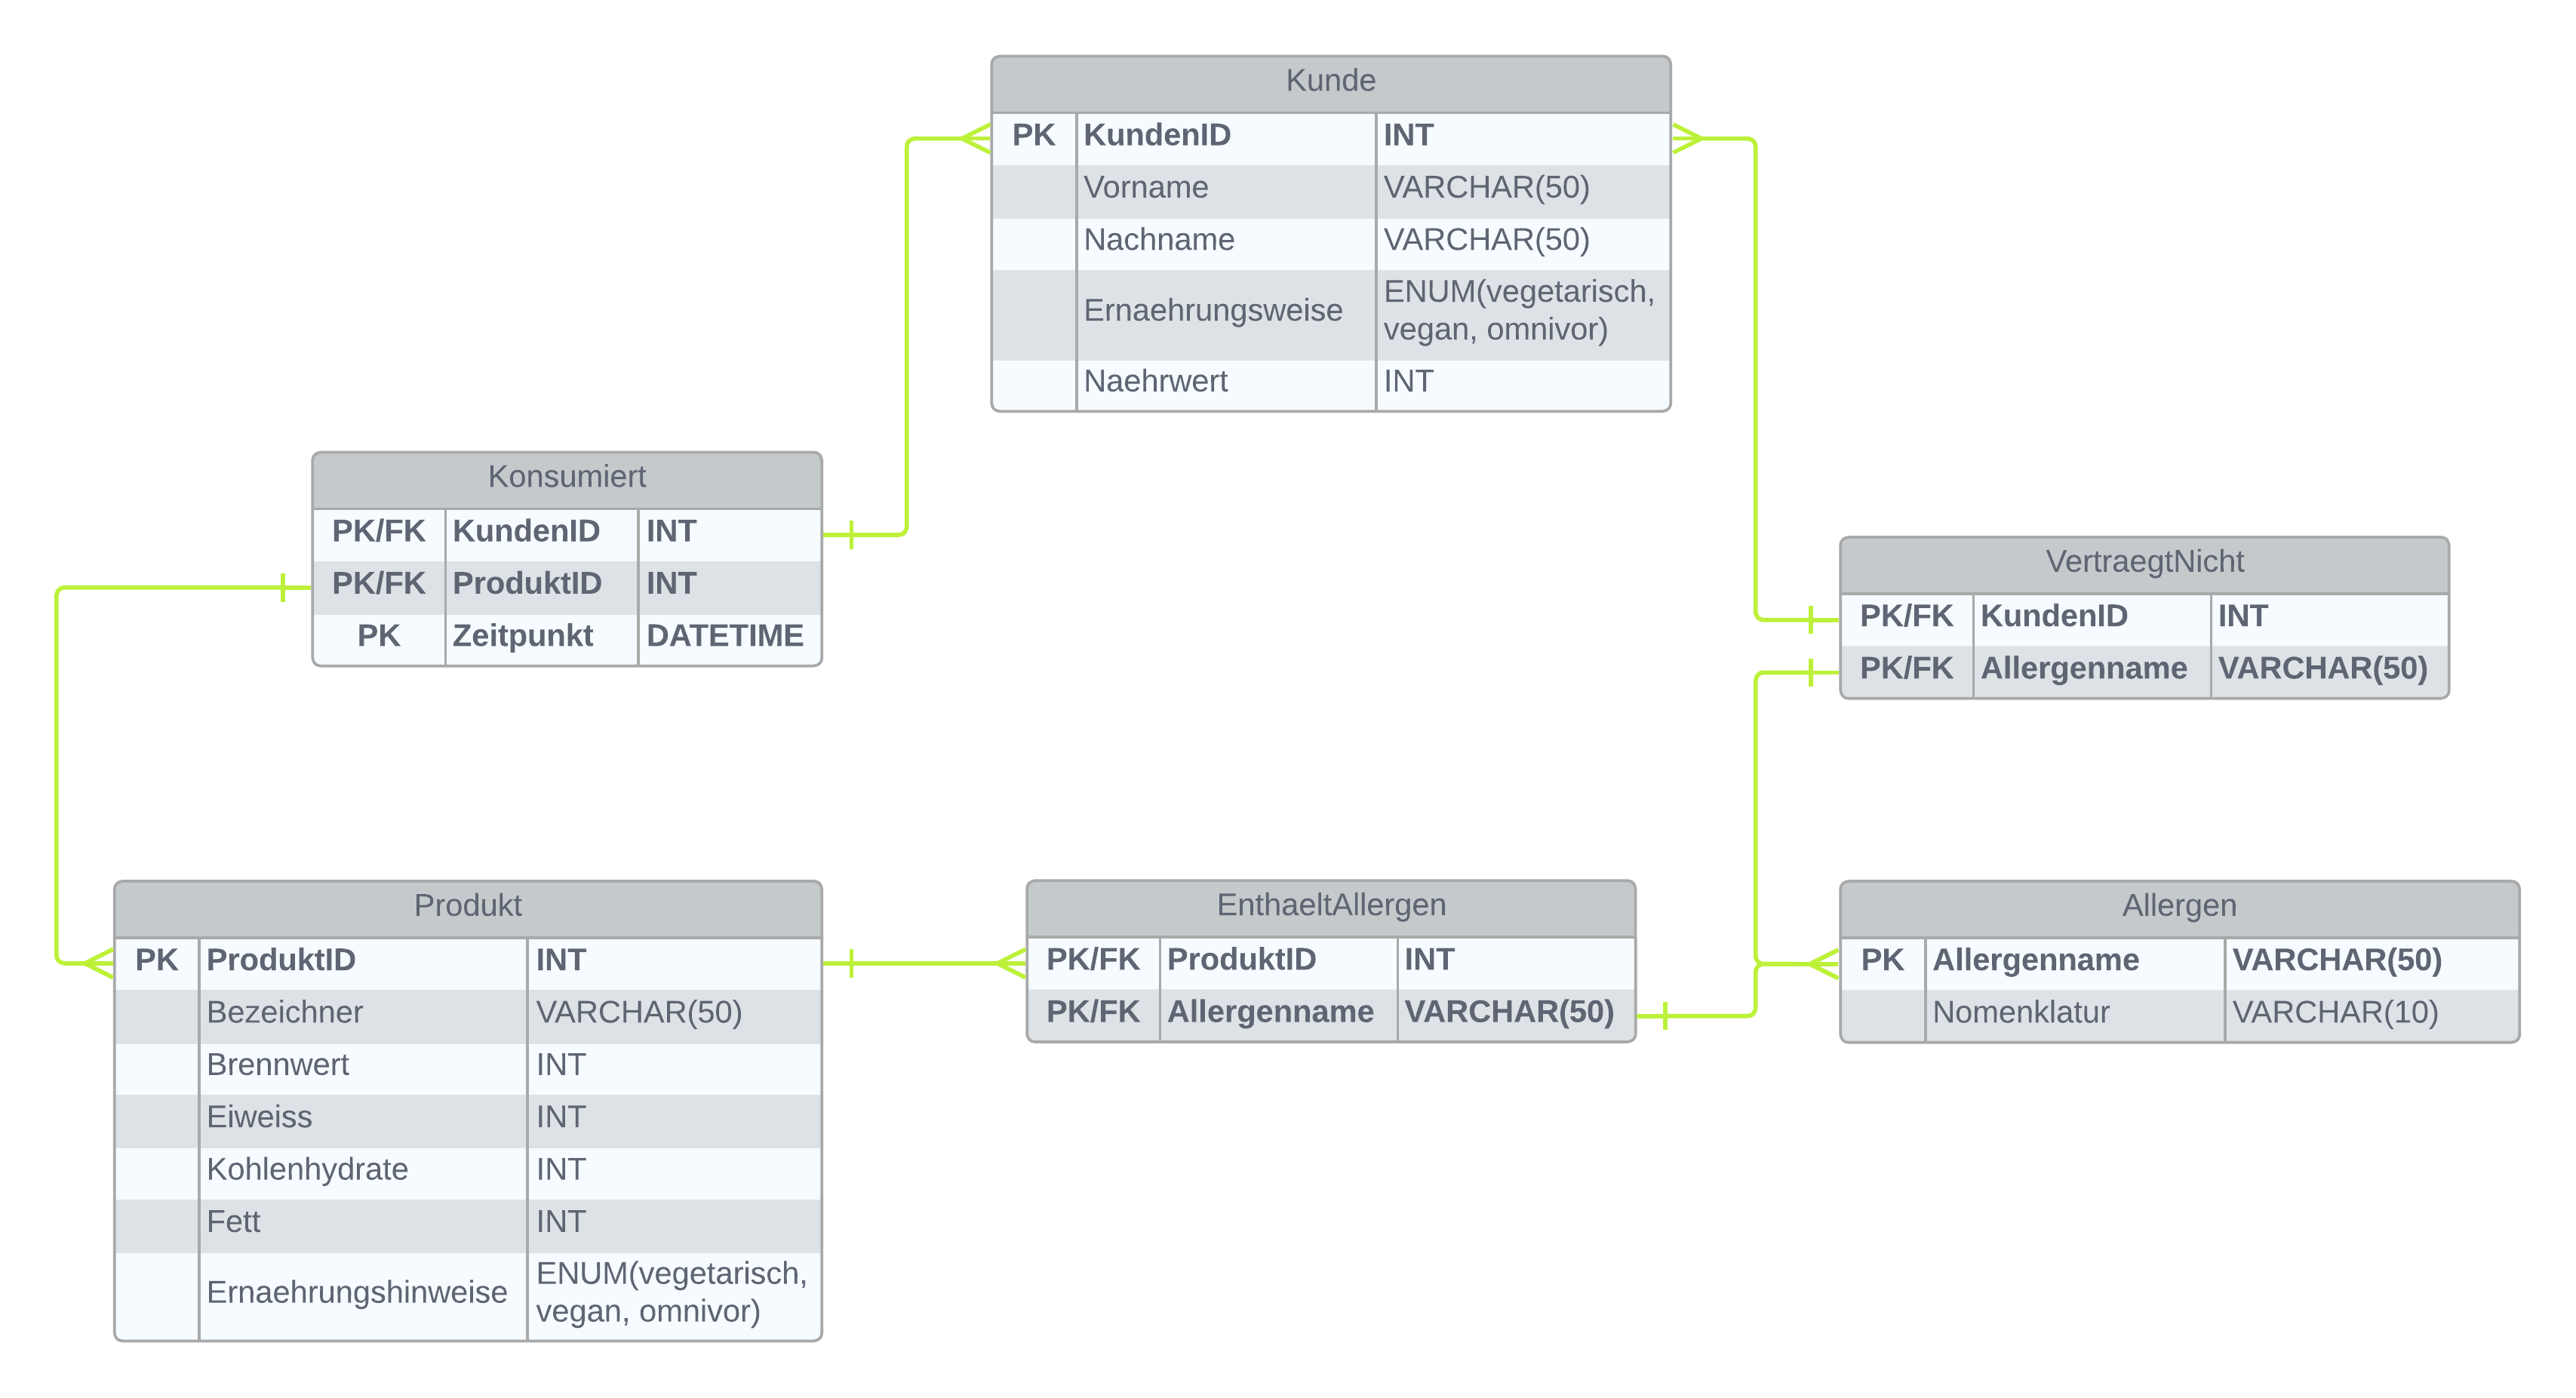
\includegraphics[width=0.9\textwidth]{images/neo4j_example_relational_model.png}
\end{figure}

\autoref{fig:relationalModelNeo4j} shows the relational model of a food consumption database. It consists of three main tables, \textit{Kunde}, \textit{Produkt}, and \textit{Allergen} that are connected by the link tables \textit{Konsumiert}, \textit{VertraegtNicht}, and \textit{EnthaeltAllergen}. The link tables are used to map the many-to-many relationships between the main tables.

The \textit{Kunde} table contains customer data, such as first name, last name, or diet. The \textit{Produkt} table stores details about the products, such as name and nutritional values. Finally, in the \textit{Allergen} table, the name and nomenclature of the allergens are stored.

As a relationship between \textit{Kunde} and \textit{Produkt}, the table \textit{Konsumiert} stores which products a customer has consumed. It also has an additional column \textit{Zetipunkt} for the consumption date. The table \textit{VertraegtNicht} contains information about the allergens that customers are allergic to. Last, the table \textit{EnthaeltAllergen} stores the allergens that are contained in products.

\subsubsection*{Graph Model}

\begin{figure}[H]
    \centering
    \caption{Graph Model of the Food Consumption Database}\label{fig:graphModelNeo4j}
    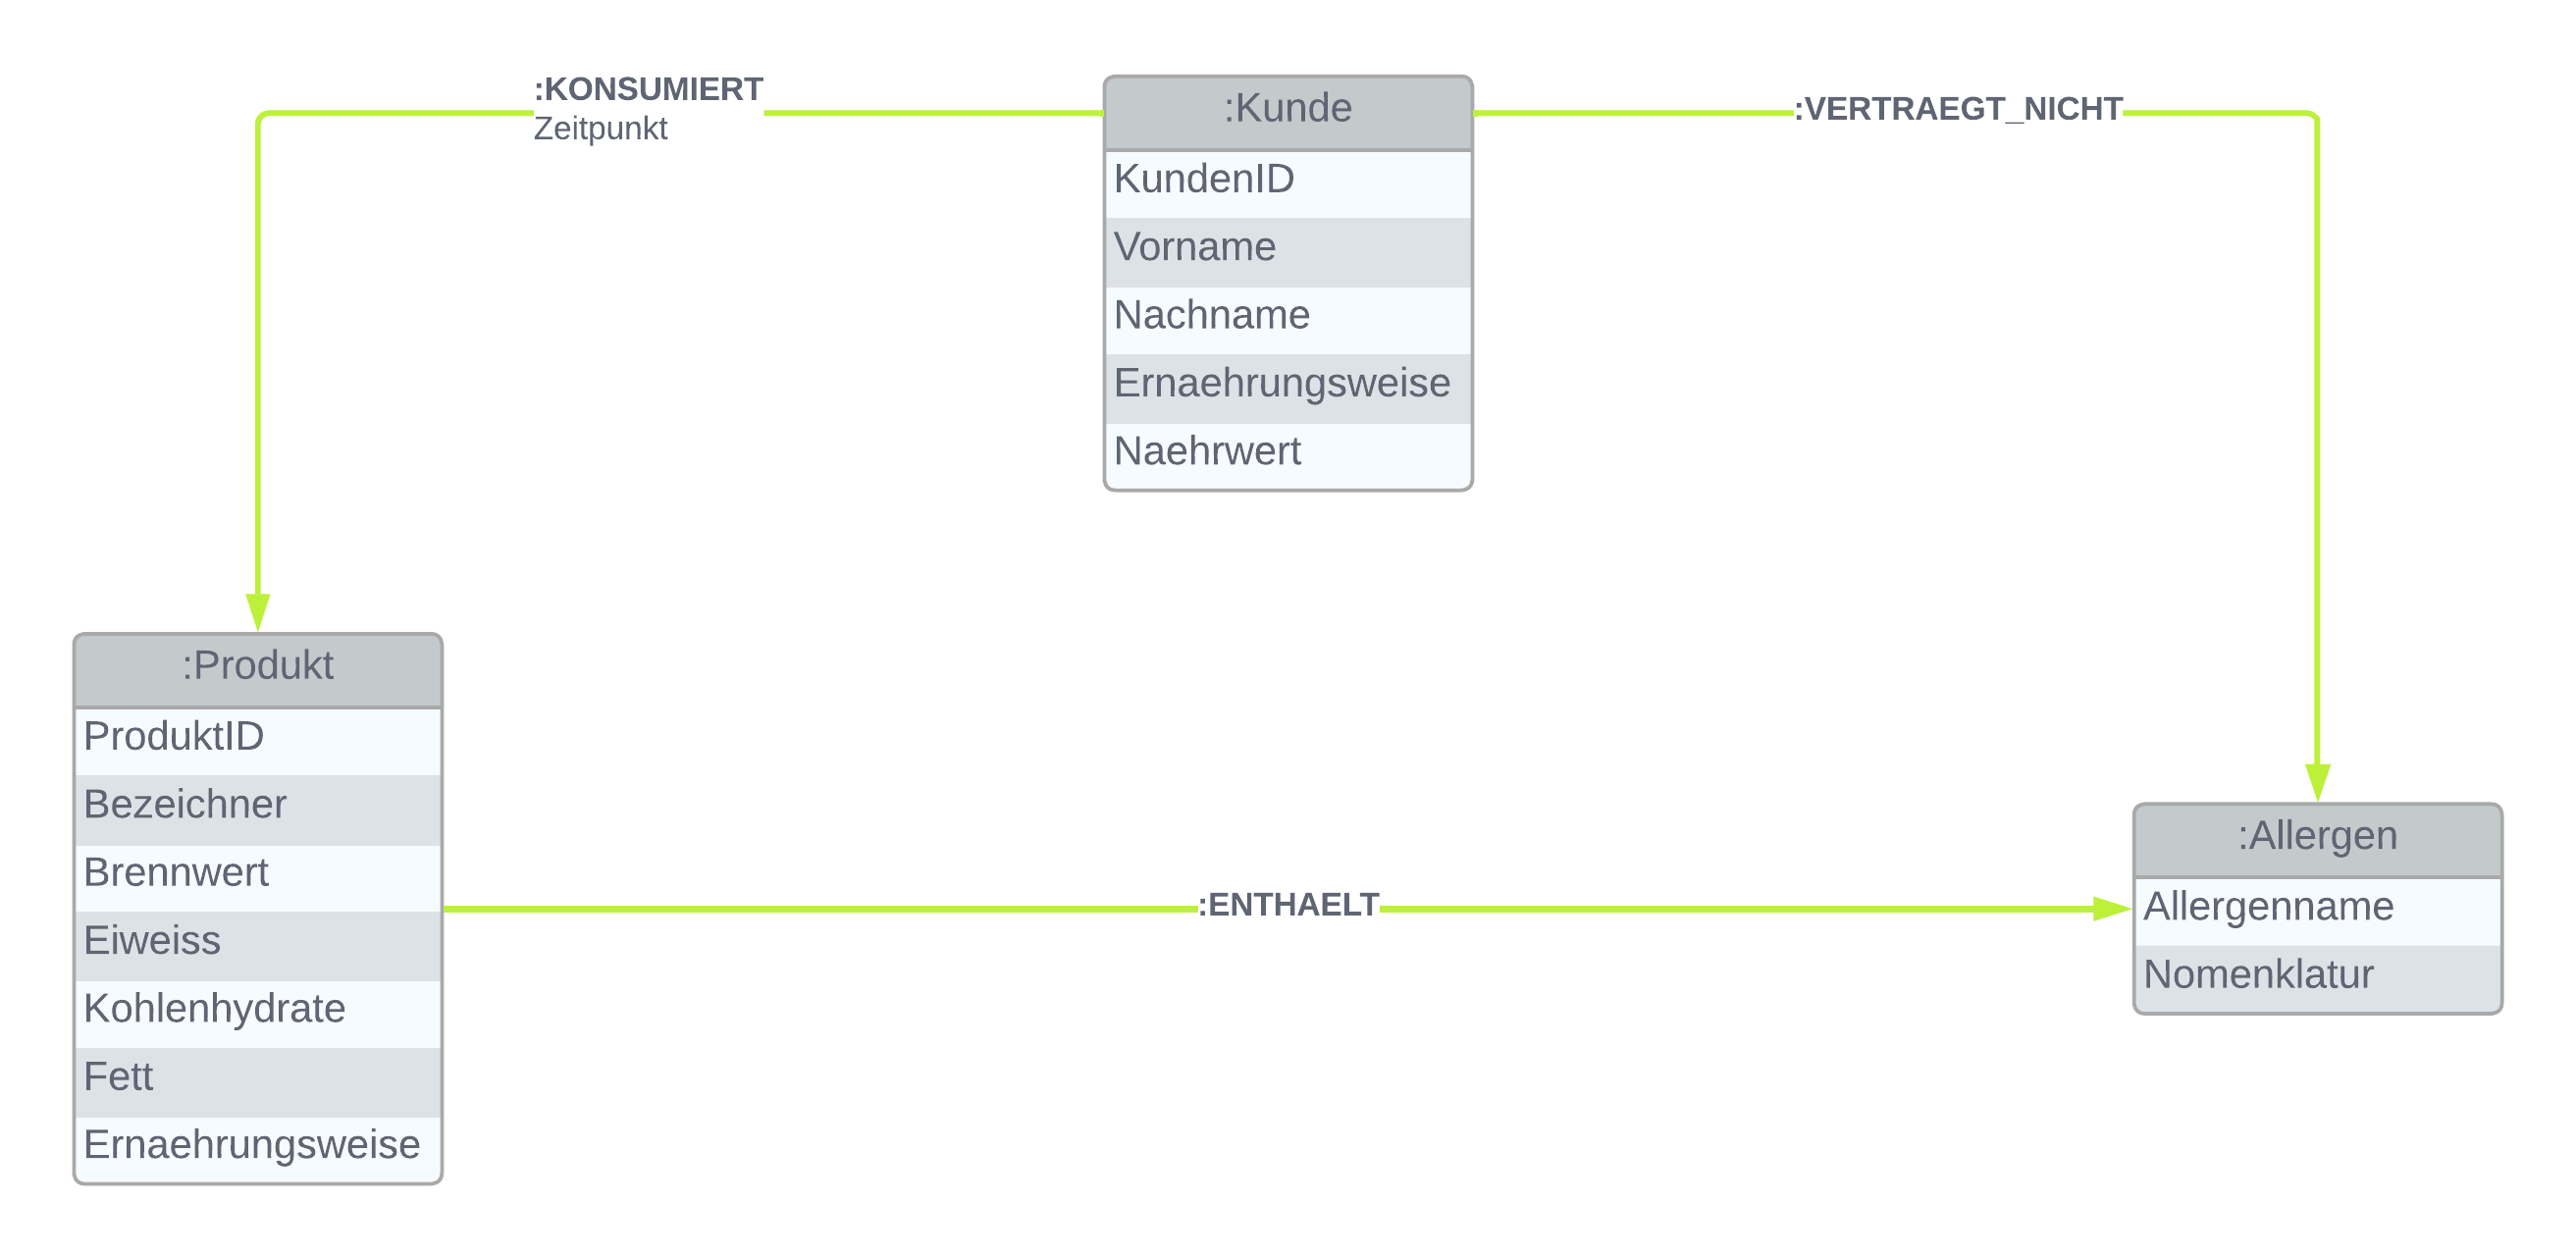
\includegraphics[width=0.9\textwidth]{images/neo4j_example_graph_model.png}
\end{figure}

\autoref{fig:graphModelNeo4j} illustrates a graph model based on the previously described relational food consumption database. The main tables \textit{Kunde}, \textit{Produkt}, and \textit{Allergen} are now represented by a specific type of node with the table name as the label. It is important to notice that in contrast to the relational model, where all data is stored in a single table, in the graph model every row of a table is represented by a distinct node. Since nodes in Neo4j can have properties, the column values of the original table can be stored as properties of the nodes.

In addition, the link tables \textit{Konsumiert}, \textit{VertraegtNicht}, and \textit{EnthaeltAllergen} are now represented by direct connections, so edges between nodes, of the entities of a relationship. For example, the relationship between \textit{Kunde} and \textit{Produkt} is now represented by an edge between the nodes of the \textit{Kunde} and \textit{Produkt} labels. The edges are labeled with the name of the relationship, in this case \textit{Konsumiert}. This edge also has a property \textit{Zetipunkt} that stores the consumption date.

\subsubsection*{Key Takeaways}

When migrating from a relational database model to a graph database model, there are several essential steps to follow, as could be noted in the previous example. These include --- most important --- the use of node labels, the mapping of table entries to nodes, the usage of relationships instead of foreign keys, and the replacement of link tables with relationships \parencite{neo4j_docs_migration}.

In a graph database model, tables from the relational model are mapped to node labels. Each node label represents an entity type that can be used to query and analyze the data. In the example of the food consumption database, the \textit{Kunde} table would be mapped to a \textit{Kunde} node label, the \textit{Produkt} table to a \textit{Produkt} node label, and the \textit{Allergen} table to an \textit{Allergen} node label.

In addition, for each row in a table, a separate node has to be created. The node is labeled with the name of the table, and the columns of the table are represented as properties of the node. In the previously shown example, a \textit{Kunde} node has properties such as \textit{Vorname}, \textit{Nachname}, or \textit{Ernaehrungsweise}, which were columns in the original relational schema.

In relational databases, one-to-one or one-to-many relationships can be expressed by adding a foreign key of one of the participating tables of a relationship to the other. However, in a graph database model, relationships can be expressed by direct connections through edges between nodes. Hence, foreign keys are not necessary anymore. Just like nodes, relationships also have a label to distinguish between different kinds. For example, a \textit{Konsumiert} relationship might connect a \textit{Kunde} node with a \textit{Produkt} node, representing the fact that the customer has consumed the product. This approach of realizing relationships enables more complex and flexible queries without the need to join tables.

Finally, for a many-to-many relationship in relational databases, there has to be a separate link table storing only foreign keys and potentially additional attributes of the relationship. In graph databases, these link tables can be replaced with relationships as well. Since relationships can have properties, any attributes of the original link table can be stored in this way. In that regard, Neo4j simplifies the data model and also eliminates the need for additional join operations that are required in relational models. In the food consumption database example, the link table \textit{Konsumiert} can be replaced by an edge between the nodes \textit{Kunde} and \textit{Produkt} with the additional property \textit{Zeitpunkt}.

\subsection{Installation} \label{subsec:installationNeo4j}

Neo4j can be installed on a local machine for personal use either via the Desktop Application (e.g., \texttt{.exe}, AppImage) or the Linux package \parencite{neo4j_neo4j_nodate}. For production environments, Neo4j can be deployed using Docker \parencite{neo4j_docs_introduction_nodate} or Kubernetes to scale the database horizontally.

As Neo4j is implemented in Java, a \ac{jdk} must be installed, although the containerized versions may already include one.

In this paper, we'll deploy a single instance of Neo4j using a Docker container. The container exposes two ports: \num{7687} for the \ac{ui} to run Cypher queries and \num{7474} for the \ac{bolt} used to communicate with the database.

\subsection{Cypher Examples} \label{subsec:queryingNeo4j}

To create nodes and query them, we'll use the graph model from \autoref{subsec:migrationRelationModelNeo4j}.

\begin{code}[H]
    \caption{Cypher Query to create a node} \label{code:cypherCreateNode}
    \begin{minted}[linenos, breaklines]{cypher}
// Create :Kunde nodes
CREATE (FelixHoffmann:Kunde {KundenID: "42", Vorname: "Felix", Nachname: "Hoffmann", Ernaehrungsweise: "vegan", Naehrwert: 1337})

// Create :Produkt nodes
CREATE (BigMac:Produkt {ProduktID: "1", Name: "Big Mac", Naehrwert: 257})

// Create :Allergen nodes
CREATE (GlutenhaltigesGetreide:Allergen {Allergenname: "Glutenhaltiges Getreide", Nomenklatur: "gluten"})

// Create :Konsumiert relationship
CREATE (FelixHoffmann)-[:Konsumiert {datum: "2019-01-01"}]->(BigMac)
    \end{minted}
\end{code}

\vspace{-\parskip}

\autoref{code:cypherCreateNode} shows a simple Cypher query to create multiple nodes and a relationship. The \texttt{CREATE} keyword starts the query, followed by a unique key for the node and the node type specified by the \texttt{:} symbol and its label. We can then specify attributes related to the node, such as \texttt{Vorname} set to \texttt{Felix} and \texttt{Nachname} set to \texttt{Hoffmann}. Lastly, the \texttt{CREATE} keyword and the relationship between two nodes are defined using an arrow syntax. The relationship label is set to \texttt{Konsumiert}, and the \texttt{datum} attribute is set to \texttt{2019-01-01}.

We then created additional nodes and relationships, resulting in the graph shown in \autoref{fig:neo4jGraph_1}. To retrieve this graph, we run the query \texttt{MATCH (n) RETURN n}, which matches all nodes in the database and returns them.

\begin{figure}[H]
    \centering
    \caption{Graph including all nodes in the database} \label{fig:neo4jGraph_1}
    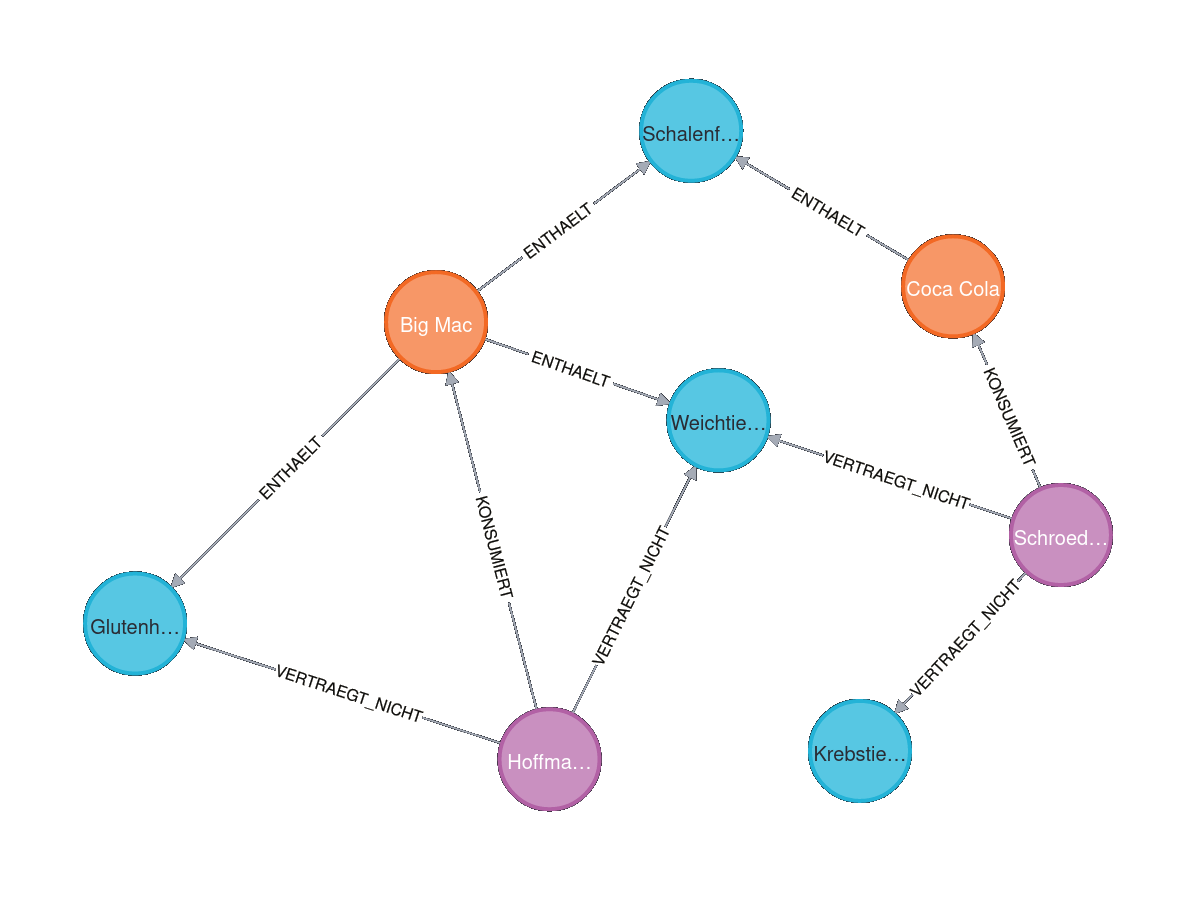
\includegraphics[width=0.7\textwidth]{images/neo4j_example_graph_1.png}
\end{figure}

For this example, we created additional nodes and relationships. The query result is shown in \autoref{fig:neo4jGraph_1}. The graph shows all nodes and relationships in the database. This graph can be retrieved by running \texttt{MATCH (n) RETURN n}. The \texttt{MATCH} keyword is used to specify the pattern of the query. In this case, we want to match all nodes in the database. The \texttt{RETURN} keyword is used to specify the result of the query. In this case, we want to return all nodes in the database.

\begin{code}[H]
    \caption{Cypher Query to select allergic reactions} \label{code:cypherFindAllergicReactions}
    \begin{minted}[linenos, breaklines]{cypher}
// Detect customer who ate a product that contains an allergen that is not able to eat
MATCH (k:Kunde)-[:Konsumiert]->(p:Produkt)
(k)-[:VERTREAGT_NICHT]->(a:Allergen)<-[:ENTHAELT]-(p)
RETURN k, a, p
    \end{minted}
\end{code}

Next, we run a query to find all allergic reactions, shown in \autoref{code:cypherFindAllergicReactions}. The \texttt{MATCH} keyword specifies the query's pattern to match all nodes of types \texttt{Kunde} and \texttt{Produkt} connected by a relationship of type \texttt{Konsumiert}. We then specify that the customer does not tolerate an allergen, and the product contains this allergen. Lastly, we want to return the customer and the product. The query result is shown in \autoref{fig:neo4jGraph_2}.

\begin{figure}[H]
    \centering
    \caption{Graph of a selection of Nodes} \label{fig:neo4jGraph_2}
    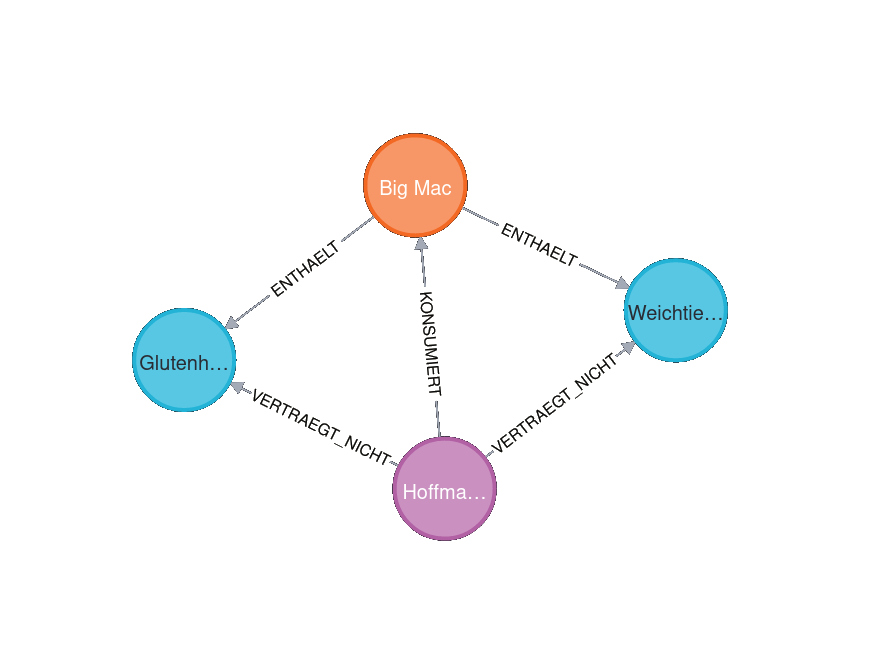
\includegraphics[width=0.6\textwidth]{images/neo4j_example_graph_2.png}
\end{figure}

\section{Reflection} \label{sec:reflectionNeo4j}

Exercitation qui duis voluptate do esse aute. Minim deserunt ex minim sunt cupidatat est fugiat in pariatur ullamco. Enim esse voluptate nulla et sunt sint labore non ut eiusmod et. Deserunt laboris ullamco occaecat esse reprehenderit anim. Deserunt aute laboris tempor est occaecat duis in cupidatat.

\subsection{CAP Theorem} \label{subsec:capTheoremNeo4j}

Exercitation qui duis voluptate do esse aute. Minim deserunt ex minim sunt cupidatat est fugiat in pariatur ullamco. Enim esse voluptate nulla et sunt sint labore non ut eiusmod et. Deserunt laboris ullamco occaecat esse reprehenderit anim. Deserunt aute laboris tempor est occaecat duis in cupidatat.

\subsection{Conclusion} \label{subsec:conclusionNeo4j}

Exercitation qui duis voluptate do esse aute. Minim deserunt ex minim sunt cupidatat est fugiat in pariatur ullamco. Enim esse voluptate nulla et sunt sint labore non ut eiusmod et. Deserunt laboris ullamco occaecat esse reprehenderit anim. Deserunt aute laboris tempor est occaecat duis in cupidatat.
